\documentclass[12pt]{article}
% This first part of the file is called the PREAMBLE. It includes
% customizations and command definitions. The preamble is everything
% between \documentclass and \begin{document}.

\usepackage[margin=1in]{geometry}  % set the margins to 1in on all sides
\usepackage{graphicx}              % to include figures
\usepackage{amsmath}               % great math stuff
\usepackage{amsfonts}              % for blackboard bold, etc
\usepackage{amsthm}                % better theorem environments

\usepackage{rotating} % for sideway table
\usepackage{xcolor}
\usepackage{hyperref}
\hypersetup{
    colorlinks,
    linkcolor={red!50!black},
    citecolor={blue!50!black},
    urlcolor={blue!80!black}
}
\usepackage{cleveref} % Reference
\usepackage{enumitem} % nosep

\usepackage{array,tabularx}

\newenvironment{conditions*}
  {\par\vspace{\abovedisplayskip}\noindent
   \tabularx{\columnwidth}{>{$}l<{$} @{${}={}$} >{\raggedright\arraybackslash}X}}
  {\endtabularx\par\vspace{\belowdisplayskip}}
  
\usepackage{float}
\restylefloat{table}

% various theorems, numbered by section

\newtheorem{thm}{Theorem}[section]
\newtheorem{lem}[thm]{Lemma}
\newtheorem{prop}[thm]{Proposition}
\newtheorem{cor}[thm]{Corollary}
\newtheorem{conj}[thm]{Conjecture}

\DeclareMathOperator{\id}{id}

\newcommand{\bd}[1]{\mathbf{#1}}  % for bolding symbols
\newcommand{\RR}{\mathbb{R}}      % for Real numbers
\newcommand{\ZZ}{\mathbb{Z}}      % for Integers
\newcommand{\col}[1]{\left[\begin{matrix} #1 \end{matrix} \right]}
\newcommand{\comb}[2]{\binom{#1^2 + #2^2}{#1+#2}}

% bibliography
\usepackage{natbib}
\bibpunct{(}{)}{;}{a}{}{,} % no comma between author and year

\title{Prospectus: The effect of corruption on FDI technological spillover}
\author{Anh Le}


\begin{document}
\maketitle

\section{Empirical Puzzle}
In recent decades, foreign direct investment (FDI) global flow has steadily increased, rising to over \$1.5 trillion dollars in 2014. For developing countries, FDI flow is also remarkably robust to global downturn, leading to enthusiastic endorsement by major international organizations as a key factor to economic development (\Cref{fig:globalfdi}) \citep{Mallampally1999, WorldEconomicForum2013}. This assumption is also shared widely within political science, where much of the literature starts with the assumption that countries want to seek FDI for its many benefits. The question that these works focus on is \textit{how} countries can attract FDI, not \textit{why} they want to do so \citep{Jensen2003, Li2003, Li2006, Ahlquist2006}.\footnote{Two recent exceptions are \citet{Pinto2013, Pandya2013}, which are the first to investigate the demand for FDI.} 

\begin{figure}[!ht]
\includegraphics[width=\textwidth, height=\textheight,keepaspectratio]{../figure/global_fdi}
\caption{FDI flow to the developing economies has been increasing steadily and proves robust to economic downturn. Source: \citet[xiii]{UNCTAD2014}}
\label{fig:globalfdi}
\end{figure}

Underlying this mode of thinking is the assumption that FDI brings various benefits to developing countries, including capital and employment. However, the more important promise that FDI holds to growth is the spillover of productivity between foreign firms and domestic firms. As well-known from neoclassical growth theory, the diminishing return to capital will at one point stop capital from accumulating further, preventing long-run economic growth from being permanently driven by capital accumulation alone \citep{Solow1956}. Therefore, long-run growth ultimately requires technological innovation, of which FDI is potentially an important source.

This insight implies that FDI cannot promote the host country's growth simply from the amount of capital it brings. Scholars have confirmed that FDI can only have a growth-enhancing impact if there is technological spillover from the foreign to the domestic sectors \citep{Nunnenkamp2004}. This empirical finding provides support for \citet{Findlay1978}'s groundbreaking model of FDI and growth, in which technology spillover from foreign firms shift the domestic factor-price frontier to the right, allowing more output from the same input, resulting in higher profits and higher wages (i.e. higher savings) for the domestic sector. This ultimately leads to a continually increasing domestic capital stock. In this view, FDI is welfare-enhancing, providing spillover benefits to the local firms in ways that foreign firms do not take into account in their private calculations. This provides the justification for countries' using investment incentives to rectify the undersupply of FDI, closing the gap between private and social returns. 

Despite this prevailing view about the importance of FDI in providing technological spillover, there is little conclusive evidence of FDI having a positive effect on growth \citep{Nair-Reichert2001, Carkovic2002} or poverty reduction \citep{Guerra2009} (\Cref{fig:fdipoverty}). A substantial literature has developed to explain this puzzle, concluding that the growth-enhancing and spillover effect of FDI is conditional on the absorptive capacity of local firms. Cross-nationally, scholars find that FDI is more likely to have a positive growth effect when the technological gap between the local and foreign firms are small \citep{Nunnenkamp2004} and when host countries have strong financial and institutional development \citep{ Durham2004}. Similarly, absorptive capacity, measured by the level of schooling in host economy, conditions the transfer of technology between foreign and local firms across regions in China \citep{Fu2008} and countries in Latin America \citep{Willem2004}.

\begin{figure}[!ht]
\includegraphics[width=\textwidth, height=\textheight,keepaspectratio]{../figure/fdi_poverty}
\caption{Relationship between FDI and poverty}
\label{fig:fdipoverty}
\end{figure}

Despite the resounding conclusion that the effect of FDI is highly conditional and that investment incentives do not work, why do countries still fixate so much on bringing in FDI \citep{Blomstrom2002}? For example, Ireland provided foreign investors with lower tax rate, lower land price, and cash grants for R\&D that do not need to be repaid. China also used a tax holiday (two years of no tax and three year of half the normal tax rate) in special economic zones to attract more foreign firms \citep{Telford2001}. We see the same widespread use of investment incentives in Southeast Asia \citep{Fletcher2002}. In Vietnam, the race to offer incentives to foreign firms rages on even among sub-national units, as provincial governments defied the central government's directive and offered extra-legal incentives to FDI firms \citep{Vu2007}. Not only do these measures not work in attracting more FDI, they also deprive countries of revenues that could be spent on improving the local labor quality and investment climate, which are much more conducive to spillover effect and growth.

Thus, my dissertation project focuses on this empirical puzzle: if the positive effect of FDI is uncertain, why is there so much focus on attracting it? To understand this puzzle, I propose that we need to take into account the calculus of government officials, who may be more interested in foreign firms as a source of private benefit rather than in the spillover and growth-enhancing effect of FDI. This is a potential reason why we often see countries (i.e. government officials) being so enthusiastic about attracting FDI, yet not so passionate about developing the local capacity that enables FDI to actually have a positive effect on growth.

\section{Tentative Evidence}
In this section, I present some stylized facts that motivate the puzzle and the hypothesized link between FDI and corruption:

\begin{itemize}
	\item The spillover effect of FDI on growth is highly variable. For example, FDI is found to be growth-enhancing in East Asia, but not in Latin America \citep{Zhang2001}. Similarly, the effect of FDI on domestic investment also varies across countries and regions. FDI is found to crowd in investment in some countries (e.g. Ghana, Senegal, South Korea, Pakistan, Thailand, etc.) but crowd out in others \citep{Agosin2005}.
	
	\item Despite the prevalent concern with discrimination against foreign firms in the international business literature, the World Bank Enterprise Survey finds that foreign firms actually face fewer obstacles than domestic firms while doing business, suggesting a collusive relationship between host governments and foreign firms \citep{Batra2003}.
\end{itemize}


\section{Generalized theory}
\subsection{Actor and choices}

The model has one strategic actor: a government official. This official has control over a certain endowment (e.g. market access, cheap labor) that is attractive to foreign firms.\footnote{I define \textit{foreign firms} as firms with over 50\% ownership belonging to private foreign individuals, companies, or organizations. In these firms, we are certain that the foreign owner has the majority stake and is responsible for the firm's action. This definition is common across business surveys and national laws, allowing us to collect a wide range of data.} Foreign firms that invest in the official's territory turn this endowment into profit via their productive activities. Firms then share the value added with the official in exchange for access to the endowment. 

Firms share the benefit with the official in the form of a two-good bundle: 1) technological spillover and, 2) private benefits (to the official). \textit{Technological spillover} is the beneficial effects of foreign firms' technological knowledge on the productivity and innovative ability of domestic firms. The official cares about the technological spillover of FDI because it is a crucial ingredient in improving total factor productivity and generating long-term growth, which in turn, brings electoral or career benefits. \textit{Private benefits} that firms offer to the official can come in many forms, both illegal (e.g. bribe, kickback) and legal (e.g. campaign finance contribution, informal network with foreign firms that leads to contracts for friends and families). The essence of the dissertation project is to determine how the official chooses the mix of these two goods, i.e. technological spillover and private benefit.

In this model, the firm does care about whether the official demands spillover or private benefits but only because firms have heterogeneous abilities in offering spillover and private benefits. For example, if a firm belongs to an industry where production is divisible, it is easier and less expensive for the firm to sub-contract local firms and create spillover. Similarly, if a firm comes from a country with little corruption, it may be less adept in dealing with the official, has to hire local agents, and thus find it more expensive to offer the same amount of private benefits than other firms that are familiar with corrupt dealings. I model this preference of firm via two parameters: the ``price'' of spillover and the ``price'' of private benefit, which the official has to consider when he demands one of the two goods from the firm. By doing so, my model is able to incorporate the firm's preference without introducing it as a strategic actor.

This model has two assumptions. First, I assume that offering spillover or private benefits does not affect the firm's utility other than through the bottom line. If we believe that firms are unlikely to have moral (or other non-financial) incentives to bring spillover or to withhold bribe, then this assumption is reasonable. 

Second, I assume that the firm is satisfied as long as its retained profit remains above the reservation level. The firm will not invest if and only if the official's demand reduces its profit to below this level. This assumption is reasonable according to the behavioral model of firms, in which firms are profit-satisficing instead of profit-maximizing \citep{Simon1959}. Granted, it is less defensible to build a model with one actor satisficing (the firm) while the other maximizing (the official). Therefore, in an extension to my project, I will model both actors as utility maximizing and use two-sided logit (TSL) to estimate their preferences. \citet{Logan1996a} has shown that the TSL corresponds to the game-theoretic college admissions model, a many-to-one matching problem that is relevant to how countries and FDI firms find their match.


\subsection{The trade-off between spillover and private benefits}

To induce spillover, governments frequently impose on foreign firms conditions such as forming a joint venture or local content requirement. These conditions constrain firms' options and their ability to optimally use their physical and management capital, reducing their revenue and profitability. Similarly, when firms are forced to offer private benefit to officials (e.g. bribes, contracts with officials' relatives), they suffer from both an upfront cost as well as the cost of uncertainty (as these private benefits are frequently informal, not transparently encoded, and thus abstruse to foreign firms). For this reason, offering officials private benefit increases firms' expenses and thus also reduces profitability. Given that firms are constrained to maintain a minimum amount of profit (akin to reservation wage) that justifies investing in the country, if a firm offers more private benefit to the official it will have to bring less technological spillover, and vice versa.

One may argue that there are foreign firms that voluntarily produce spillover and this is not mutually exclusive from offering private benefit to the officials. However, such cases are rare because high-tech firms want to keep their technology proprietary. Due to scale and sophistication, foreign firms would also source from established international suppliers and only rely on local suppliers for standard commodity goods at arms-length, which doesn't generate as much spillover as personal contact (e.g. training, quality assurance assistance, financing assistance). FDI firms voluntarily source from local suppliers only when the availability and quality of local suppliers are not far from international quality, and in these cases there's less need and room for spillover. Another scenario that leads to foreign firms voluntarily producing spillover is when they specifically target the local market: in this case, the qualilty requirement is not too stringent, the quantity not too large, and there is a need for rapid local customization. However, in this case, market oriented FDI firms can displace local firms, and the benefit of spillover is offset and can lead to negative spillover \citep{Mody2004}.

Given that offering either spillover or private benefits cut into the firm's profit, and that the firm's profit is finite, the official can only have more of one good if he has less of the other. In other words, there is a trade-off between spillover and private benefits, and the official faces a budget constraint over this two-good bundle.

While FDI does bring other benefits, e.g. jobs and capital, the theory intentionally focuses on technological spillover and private benefits for both substantive and theoretical reasons. Substantively, technological spillover increases total factor productivity, which is key to sustaining long-term economic growth when capital has diminishing return. While the literature has mainly focused on the quantity of FDI attracted, development agencies and governments have paid much attention to the issue of technological spillover. 

Furthermore, the implication of a spillover-vs-private-benefit trade-off is very different from that of a spillover-vs-capital/job trade-off. In the later case, one can count on the official to shift towards attracting FDI with high technological spillover as his country gradually grows and is in less immediate need of capital and job creation. The growth trajectory of a country is guaranteed to be positive in this scenario, fueled by FDI's capital injection in the earlier stage and sustained by FDI's technological transfer in the later stage. However, if the trade-off that the official considers is between spillover and private benefit as my project theorizes, then one cannot count on the official to take such benevolent action.

Theoretically, since technological spillover is key to growth, my theory about the official choosing the spillover-vs-private-benefit bundle speaks to the age-old research question: ``Why are some governments corrupt, some growth-promoting, and yet others are both?'' While such question is massive both in its importance and its difficulties, my project approach FDI's spillover effect as a mid-size problem with several mid-level theories, where the model of an official considering the mix of benefits brought by a FDI project is not too abstract from the real-world investment process to be fictional. With the theory well delineated within the topic of FDI, we can pinpoint the parameters that affect the budget constraint and the official's preference over spillover and private benefit as follows.

\subsection{Parameter 1: Official's endowment determines the size of the budget constraint}

Since the official uses his endowment to attract FDI, greater endowments will engender both more technological spillover and more private benefits. In other words, his budget constraint will shift to the right (\Cref{fig:budget_constraint}). This feature of the model captures the fact that officials in a country with a lot of endowment have a much better bargaining leverage vis-a-vis the foreign firms and can extract both spillover and private benefit (e.g. China).

\begin{figure}[!ht]
	\centering
    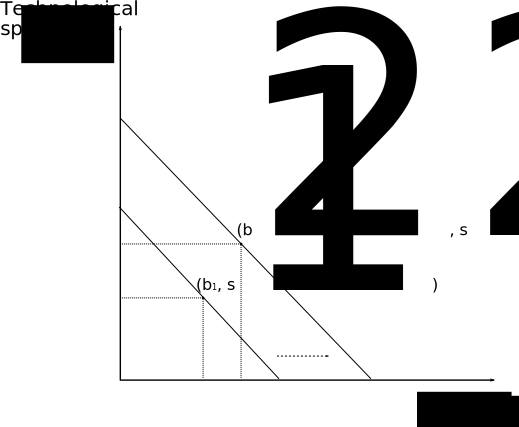
\includegraphics[width=0.75\textwidth, height=0.75\textheight,keepaspectratio]{../figure/budget_constraint}
    \caption{When an official has more endowment, his budget constraint shifts from left to right. He is now able to afford the $(s_2, b_2)$ bundle, with $s_2 > s_1$ and $b_2 > b_1$.}
    \label{fig:budget_constraint}
\end{figure}

\subsection{Parameter 2: price of spillover and private benefit determines the intercept and the slope of the budget constraint}

Given a fixed amount of endowment, the two intercepts of the budget constraint are determined by the ``price'' of the two goods, i.e. how easily the official can obtain technological spillover and private benefit from the foreign investors. If a good becomes harder to extract from foreign firms, the official can afford less of it and the corresponding intercept shifts inward (\Cref{fig:relative_price}). Alternatively, we can think of the slope of the budget constraint as the relative price of the two goods.

Substantively, the ``price'' of technological spillover depends on both the nature of the sector as well as the absorptive capacity of the local economy, which I define as the presence of private firms that are able to absorb technology from foreign firms.\footnote{I define \textit{private firms} as firms with over 50\% ownership belonging to private domestic individuals, companies, or organizations} Consider two channels through which technological spillover happens. First, private firms enter into the supply chain of foreign firms, improving their productivity by imitating the higher production standards or management techniques of foreign firms. For this to happen, it is necessary to have a wealth of private firms that are technologically capable to enter the supply chain. The feasibility of such outsourcing is also sector-specific, e.g. whether the production process is divisible into units, or whether the technology has matured enough for subcontracting. Second, local employees employed by foreign firms may learn from their experience and transfer that knowledge when they move to private firms. For this to happen, private firms must also be technically advanced enough to make use of and compete for this high quality labor from the foreign sector.

The ``price'' of private benefit substantively means how easily the government officials can extract these benefits from the foreign firms. One example of such parameter is the origin of the foreign firm. Firms that come from countries where corruption is more common or accepted would be more adept at providing private benefit to official and more willing to do. In contrast, firms from countries that have signed onto the OECD anti-bribery convention would be more hesitant to bribe given the punishment that they may face from their home governments.

Changing prices of the two goods will shift the budget constraint and, holding the indifference curve constant, have implications for the mix of two goods that the official chooses.

\begin{figure}[!ht]
	\centering
    \includegraphics[width=\textwidth, height=\textheight,keepaspectratio]{../figure/absorptive_capacity}
    \caption{In the left panel, the intercept for private benefit moves from the right to the left as its price increases. In other words, $\frac{E}{p_{b2}} < \frac{E}{p_{b1}}$ because $p_{b2} > p_{b1}$. Similarly, in the right panel, as it becomes more difficult to extract spillover from foreign firms, the intercept moves down.}
    \label{fig:relative_price}
\end{figure}

\subsection{Parameter 3: The official's time horizon determines the shape of his indifference curve}

The official has a convex indifference curve, meaning that there is decreasing marginal utility to both spillover and private benefit. This assumption is standard and makes intuitive sense. As the official accumulates more private benefit, there are fewer things worth spending on as his consumption is satiated and produces less utility. Similarly, when more technological spillover happens, it becomes less of a bottleneck to the economy. Thus, voters (or the official's higher-ups) become less concerned with the issue and it brings less electoral (or career) benefits.

The shape of the indifference curve denotes the relative weight the official assigns to the two goods, spillover and private benefit. When the curve is steep, it means that the official is willing to trade a lot of spillover for a small increase in private benefit. Vice versa, a flatter curve indicates that the official values spillover more (\Cref{fig:indifference_curve}).

Politically, the steepness of the indifference curve depends on the time horizon of the official. This is because technological spillover takes time to happen and increase economic growth whereas private benefit is immediate. The longer the time horizon, the more heavily does he weigh technological spillover effect. For example, in \Cref{fig:indifference_curve}, the blue indifference curve is flatter and signifies more weight assigned to spillover. In that case, the official chooses a bundle that has more spillover and less private benefit (i.e. $s_1 > s_2$ and $b_1 < b_2$). Political factors that influence the official's time horizon may include term limit, the stability of the regime, or the probability of electoral success. 

\begin{figure}[!ht]
	\centering
    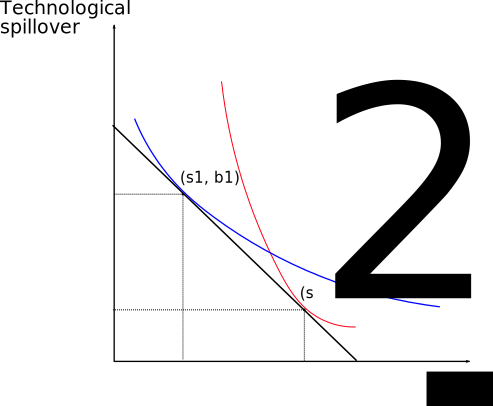
\includegraphics[width=0.75\textwidth, height=0.75\textheight,keepaspectratio]{../figure/indifference_curve}
    \caption{The blue indifference curve shows that the longer the official's time horizon, the flatter his indifference curve, and he will choose more spillover and less private benefit.}
    \label{fig:indifference_curve}
\end{figure}

\subsection{Literature on corruption and FDI}

Regarding private benefit for the officials, I focus on corruption, i.e. bribe and informal fees, given the ubiquity of the practice in developing markets and wealth of data collected on this issue from cross-national business surveys. 

The majority of literature on the relationship between corruption and FDI focuses on showing that a high level of corruption deters FDI \citep{Wei2000, Hakkala2008, Al-Sadig2009}. A smaller literature examines the behaviors of foreign firms that choose to invest in a highly corrupt environment. It argues that foreign firms can help reduce corruption in host country via regulatory pressure effect, demonstration effect, and professionalization effect \citep{Kwok2006}; or via competing away the rents of the domestic firms, reducing the supply of bribes \citep{Sandholtz2003}. In these works, corruption between the host government and the foreign firm has been conceptualized as \textit{predatory}.

My research offers a new perspective, recognizing that, compared to domestic firms, foreign firms always have the freedom to move out of the country or at least stop bringing in capital. Therefore, the exchange between the government and foreign firms are always more voluntary compared to private firms. In this angle, corruption between the government and the foreign firm can be \textit{collusive}, with government officials getting bribe and foreign firms getting exclusive access to resources controlled by the officials (e.g. an expedited bureaucracy or privileged use of public resources) \citep{Hellman2002}. Indeed, there are evidence of foreign firms bribing to get an upper hand in the local market \citep{Barstow2012} or to pursue rent in protected industries \citep{Malesky2015}. 

Such collusive corruption between the government and foreign firm can be the key to explain the puzzle why governments may want to attract a lot of FDI despite the lack of developmental impact. (Corrupt) institutions matter, but not only to \textit{how much} FDI a country can attract as the literature has studied, but also \textit{which kind}.


\subsection{Road map}

In the sections that follow, I contextualize the general theory presented above, building three mid-level theories that map each of the three parameters to a specific empirical context. I also briefly discuss the identification strategy, leaving more operationalization and data availability details for the later Research Design section.

The three parameters in the model and their empirical implications are:

\begin{itemize}
\item \textit{``price'' of spillover}: sectoral and industry variation in the level of potential spillover affects the official's choice of the spillover-bribe bundle.

\item \textit{``price'' of private benefit}: Phase 3 enforcement of OECD's anti-bribery convention makes firms from member countries more hesitant to bribe, raising the cost of bribery and resulting in less bribe and more spillover.

\item \textit{time horizon}: term limit reduces the time horizon of Vietnamese provincial officials that are close to retirement, leading to less spillover and more bribery.
\end{itemize}

\section{Theory}
My theory aims to explain the lack of technological spillover from foreign firms to private firms. I define foreign firms as firms with over 50\% The argument will be laid out in three steps:

\begin{enumerate}
\item I argue that for FDI to have a growth enhancing effect, there must be technological spillover from foreign firms to private firms. Therefore, if we see that there is little technological spillover, it must mean that the government is attracting FDI for reasons other than growth.

Measuring technological spillover:
\begin{itemize}
\item Frequency of contacts between foreign and private firms (cite literature on spillover happen through contact here)
\item The actual increase in productivity and technological capability of private firms
\end{itemize}


\item I argue that corruption (i.e. bribes from foreign firms) is one reason (besides growth) that the government wants FDI for. The testable implication is that corruption countries (sectors) is associated with a lack of technological spillover between foreign and private firms in that countries (sectors). At this step, the level of corruption in a country (sector) is treated as exogenous.

For this argument to be convincing, one must take into account alternative explanations, i.e. reasons besides corruption and growth that governments may want FDI for:
\begin{itemize} 
\item Employment: under strong pressure for employment generation, the government may want FDI purely for the jobs it brings instead of the long-term economic growth. To account for this alternative explanation, I will control for the growth rate of labor force. Since the labor force growth is largely determined 18-20 years prior, it is plausibly exogenous to other variables in the current period and thus well-behaved statistically.  
\item Capital: In the early-stage of development, a country may deliberately pursue a capital-driven instead of technology-driven growth. To account for this alternative explanation, I will control for the aggregate capital stock or the national savings rate.
\item Election cycle: Much research has shown that the election calendar puts populist pressure on the government, leading to manipulation of macroeconomic factors such as the exchange rate \citep{Blomberg2001}. Similarly, one may argue that the government wants to attract many FDI projects for a positive headline near election time even though these projects do not have a large impact on long-term growth. To account for this alternative explanation, I will control for whether a FDI project begins in an election year.
\end{itemize}

\item I endogenize the choice of government officials to engage in corruption by explicitly considering their utility maximization. To get a handle on the options available to the officials, I hold the political system constant by focusing on the case of Vietnam. With its provincial variation in FDI attraction and private sector development, Vietnam's provinces serve as an insightful microcosm of the cross-national differences. I argue that, in Vietnam, whether there is spillover between the foreign and the private sector depends on the choice of provincial officials to choose between potential rents brought by foreign firms and promotions by the central government, of which private sector development is an important criterion.
\end{enumerate}

\subsection{The growth enhancing effect of FDI depends on spillover of technology}

As well-known from neoclassical growth theory, the diminishing return to capital will at one point stop capital from accumulating further, preventing long-run economic growth to be permanently driven by capital accumulation alone \citep{Solow1956}. Therefore, long-run growth ultimately requires technological innovation, which continually increases the productivity of capital and counteracts the diminishing returns.

This insight implies that FDI cannot promote the host country's growth simply from the amount of capital it brings. This explains the uncertain impact of FDI on growth and poverty reduction \citep{Nair-Reichert2001, Carkovic2002, Guerra2009}. Indeed, scholars have found that FDI can only a growth-enhancing impact if there is technological spillover from the foreign to the domestic sectors \citep{Nunnenkamp2004}. This empirical finding provides support for \citet{Findlay1978}'s model, in which technology spillover from foreign firms shift the domestic factor-price frontier to the right, allowing more output from the same input, resulting in higher profits and higher wages (i.e. higher savings) for the domestic sector. This ultimately leads to a continually increasing domestic capital stock.

As economists attempt to improve neoclassical growth theory by endogenizing technological progress, FDI researchers similarly investigate how technology spillover from FDI may happen instead of assuming its inevitability \citep{Romer1994}. Several channels for spillovers have been proposed.

These channels are:
\begin{itemize}
	\item imitation:  private firms may reverse engineer a production or management technique \citep{Wang1992}, which is facilitated by backward linkage between local and foreign firms \citep{Javorcik2004}. This motivates my first measure of spillover effect: \% of private firms that participate in contracts with foreign firms.
	\item competition: similar to the effect of competition from arm's length trade on productivity, the presence of foreign firms in the domestic market put pressure on local firms to reduce inefficiency \citep{Glass2002}. (Doing Business has firm-level data on the number of private/state/foreign competitors in the last year)
	\item export demonstration: foreign firms are more knowledgeable about exporting, which involves high fixed cost to set up a distribution and transport infrastructure, or learning about foreign taste and regulatory environment. Domestic firms can learn this ``export know-how'' from foreign firms \citep{Aitken1997}. This motivates my third measure of spillover effect: \% of private firms that export.
	\item skills acquisition: workers trained in foreign firms bring along their human capital when they move to domestic firms \citep{Djankov2000}. This presumes a healthy domestic sector that can offer competitive wages to workers.
\end{itemize}

Among these channels, \textit{imitation} and \textit{export demonstration} forms the theoretical basis of my measurement of spillover.

\subsection{FDI and corruption (cross-nationally and cross-sectorally)}

\subsubsection{Defining corruption}

Defining corruption has been a long-standing and inconclusive debate (cite). The contention stems from the normative nature of the ``corruption'' concept, which shifts significantly across context and thus difficult to build an analytical edifice upon. 

Consider the most common definition of corruption as ``the abuse of the public role for private gains.'' Make no mistake, this definition is not always clear cut. What constitutes ``abuse''? The term implies the violation of certain standards, which only further asks: what standards are supposed to be adhered to? Some scholars may emphasize a set of standards based on formal law, but the law is not always legitimate (cite). Yet others argue for a set of standards based on norms, but difference in norms across societies may be so extensive and unsystematic that a cross-country analysis untenable. Indeed, nepotism and cronyism in one society may be social capital in another, with all shades of favoritism in between (cite Understanding Corruption). 

In addition, the distinction between ``public'' and ``private'' are not always clear, especially during rapid economic liberalization and privatization. As the rules change continuously, the dividing line between an innovator and a rule-breaker is but a thread left blowing in the political wind (cite China's corruption book).

Mindful of this definition's shortcomings, I still choose to define corruption as the ``abuse of public role for private gains'' in my research. This is because while this definition may fail as a universal classification of corrupt act, within the scope of my research project its unclarities are largely resolved. First, regarding the potential unclarity over ``abuse'', I will focus on a law-centric definition of violation because of its precision, stability, and broad coverage. The legitimacy of the ``law'' is not as big of a concern as the countries in the sample have sovereignty over their territory and their law has a binding impact in their economic life, especially the formal sectors in which foreign firms operate. (List the countries in the doing business survey, and whether any of them is a failed state). In addition, a law-centric definition fits well with the way corruption is often framed in business surveys, my main source of data, as ``paying informal fees.'' Regardless of whether the respondents think these fees are legitimate or not, it is clear to both the officials and the firms whether these fees are official, as documented in formal laws.

Second, the ``public'' and ``private'' divide is also clear cut within the scope of my project. I focus on corrupt acts in the context of officials exchanging public resources under their control for bribes from foreign firms, for example, expedited paper work, access to land, and harass-free inspections. It is clear that these public resources and services should be distributed fairly, and that the payments are going to the officials' private wealth instead of the state's coffer.

\subsubsection{The relationship between corruption and FDI}

My hypothesis that host country officials engage in corruption with foreign firms to the detriment of domestic firms is a novel contribution to the IPE literature of FDI and corruption. So far, the literature has been predominantly dominated by studies showing that a high level of corruption deters FDI \citep{Wei2000, Hakkala2008, Al-Sadig2009}. (Summarize a bit here) But what about firms that choose to invest in a highly corrupt environment nonetheless? One strain of the literature argues that foreign firms can help reduce corruption in host country via regulatory pressure effect, demonstration effect, and professionalization effect \citep{Kwok2006}; or via competing away the rents of the domestic firms, reducing the supply of bribes \citep{Sandholtz2003}. In these works, corruption between the host government and the foreign firm has been conceptualized as \textit{predatory}.

My research offers a new perspective, recognizing that, compared to domestic firms, foreign firms always have the freedom to move out of the country or at least stop bringing in capital. Therefore, the exchange between the host government and the foreign firm will always have a \textit{voluntary} element.\footnote{There is an argument about FDI being harder to relocate, and thus subject to creeping expropriation. However, corruption doesn't tend to change that quickly, and a foreign investor looks into a country knows relatively well the level of corruption that they are getting involved with.} Through this angle, corruption between the government and the foreign firm can be \textit{collusive}, as governments get bribe while foreign firms get advantages over domestic firms in terms of an expedited bureaucracy or privileged use of public resources \citep{Hellman2002}. Indeed, there are evidence of foreign firms bribing to get an upper hand in the local market\footnote{http://www.nytimes.com/2012/04/22/business/at-wal-mart-in-mexico-a-bribe-inquiry-silenced.html?pagewanted=all} or to pursue rent in protected industries \citep{Malesky2015}. Such collusive relationship between the government and foreign firm may be the key to explain the puzzle of governments wanting to attract a lot of FDI despite the lack of developmental impact.

\subsubsection{The model of interaction between foreign firms and officials}

The sequencing of the game is as follows:
\begin{enumerate}
\item At the start of the game, the level of corruption in a country (sector) is given.\footnote{This assumption is not totally unreasonable. High level of corruption in a country may be largely the result of a political system that fails to produce accountability. Such political system is more likely to be the cause than the result of the maltreatment of domestic firms. Similarly, high level of corruption in a sector may be largely due to the nature of that sector, e.g. resource-intensive, high fixed cost leading to natural monopoy, etc. which is exogenous.}
\item  If the level of corruption is high, the government is mainly interested in FDI as a source of rent, not as a source of growth. There are several reasons why the government is interested in seeking rent from FDI firms instead of domestic firms. First, if foreign firms are more profitable than domestic firms, they have more rent to be extracted. Second, if foreign firms are larger than domestic firms, they facilitate coordination and allow corruption to be better kept secret among fewer actors. Third, if the interests of firms and the government misalign in the future, foreign firms have both the options of ``exit'' and ``voice'', whereas domestic firms only have ``voice''. The government would much prefer an exiting foreign firm to a domestic firm voicing its interest. The first and second reasons also indicate that my theory is most applicable when the entering FDI firms are large.
\item The foreign firm weighs the cost of corruption against the benefits of entering the country (sector), such as natural resource, local market, or cheap labor. If the benefit outweighs the cost, the firm enters the country (sector).\footnote{\Cref{fig:fdi_corruption} shows that among countries with a lot of FDI, the level of corruption runs the full gamut. This confirms that foreign firms often enter a country despite the cost of corruption.}
\item Since the government brings in the foreign firm for rent, not for spillover, it does not care about the development of the private sector in this country (sector). Therefore, we will see a gap in the treatment by the government of the domestic firm versus the foreign firm in this country (sector).
\end{enumerate}

The theory leads to two testable hypotheses:

(ADD MORE TESTABLE HYPOTHESIS about the intermediate process here)

\begin{quote}
Hypothesis: The presence of large FDI firms in corrupt countries is associated with a lack of technological spillover in those countries.
\end{quote}

\begin{quote}
Hypothesis: The presence of large FDI firms in corrupt sectors is associated with a lack of technological spillover in those sectors.
\end{quote}

\subsection{Endogenizing government officials' decision to engage in corruption with foreign firm}

The theory in the previous section starts with the level of corruption as a given parameter. To advance the theoretical contribution even further, it is important to endogenize the decision by the government officials to engage in corruption with foreign firm. However, ``why is a country corrupt?'' is a big and difficult question to study with a cross-national design due to an insurmountable degree of endogeneity. 

To get a handle on this question, we need to know the utility calculation of the government officials, which in turn requires knowing the options offered to the officials by the country's political economic system. Therefore, in the next step of the theory, I focus on the case of Vietnam, whose sub-national variation in FDI flow and private sector development serves as an excellent testing ground.

In addition, a cross-national study of corruption suffers from well-known conceptual and measurement issues. Conceptually, corruption means different things in different countries \citep{Rosen2010}. Empirically, even if we restrict corruption to a narrow but clear-cut definition, i.e. the act of bribery in exchange to public goods that should be equally available, it is still very difficult to measure corruption well due to sensitivity bias in surveys. Focusing on the case of Vietnam does not only keep constant the locale-dependent definition of corruption but also takes advantage of a survey list experiment conducted by \citet{Malesky2015} to accurately measure the level of corruption across provinces and sectors without sensitivity bias.

The theory is as follows. I argue that the key to the variation in provincial rent seeking of FDI is the principal-agent relationship between Vietnam's central and the provincial governments. Since most FDI projects are approved at the provincial level, it is the provincial government, not the central, that holds valuable services for sale to foreign firms. This is especially true because the implementation of central law varies widely across sub-national units in Vietnam \citep{Meyer2005}.\footnote{Vietnam's sub-national variation in implementation generalizes well to other developing countries \citep{Thun2006}} The central government, therefore, is more removed from direct contact with FDI firms and thus less likely to benefit from corruption than provincial leaders. At the same time, the central government is much more concerned with overall economic growth, which is central to the longevity of the regime \citep{Malesky2008}. Therefore, the central government is more interested in the spillover effect of FDI, which necessitates the development of a strong domestic sector as discussed.  On the other hand, each provincial leader is incentivized to free-ride on the developmental effort of other provinces and of the central to keep the entire regime stable. 

In conclusion, provincial leaders care more about private rents from FDI. In contrast, central leaders care more about the spillover effect of FDI on private sector development.

Fortunately for the central government, the principal-agent problem in this context is partially solved because monitoring is not too difficult. Indeed, the central government can observe the economic performance of the provinces and use personnel management to punish and reward provincial officials \citep{Sheng2007, Li2005}.\footnote{\citet{Shih2012} recently argue that economic performance does not matter to cadre promotion. However, they investigate all members of the Chinese Central Committee, including the central party apparatus, the army, and the central economic bureaucracy. These actors are not the important decision-makers in our theory.} Therefore, the principal-agent problem is only severe when the provincial officials are not interested in further promotion to the central government. This suggests that there will be a variation in private sector development across provinces according to the provincial officials' interest in promotion. By looking at this variation in the career interest of provincial officials, my theory contributes a fresh angle to the current literature on the relationship between decentralization and corruption, which has only postulated a one-way relationship: either decentralization increases bribery \citep{Fan2009} or reduces it \citep{Guerra2009}.

The sequencing of the game is as follows:
\begin{enumerate}
\item At the start of the game, the endowment of a province is given.\footnote{The assumption that the endowment is exogenous is reasonable. First, if it is the kind of endowment that cannot be affected by past provincial policies, e.g. natural resources, proximity to market, then it is truly exogenous. Second, even if it is the kind of endowment that can be affected by past policies, e.g. quality of the labor force, infrastructure quality, etc., it is usually good for both foreign and domestic firms. Therefore, at the start of the game, there is not yet any discrimination between foreign and domestic firms.}
\item The provincial official observes his endowment and calculates his current wealth, i.e. the return of rents from FDI firms.
\item The provincial official calculates the return of pursuing a promotion, which is a ``gamble'' with uncertainty:

the return of pursuing a promotion $=$ the return of the promotion $\times$ the probability of getting the promotion $(p)$

$p = p_0 + p_1$, with $p_0$ being the base chance of getting the promotion, and $p_1$ being the added chance if the official decides to develop the domestic sector as the central government desires.

\item The provincial official has to decide between keeping his current wealth (i.e. seek rents from FDI) or gambling (i.e. focus on private sector development to get a $p_0 + p_1$ chance of getting the promotion). Assuming that the official is risk averse, he prefers a small gamble over a large one. In this way, the base chance $p_0$ matters. If $p_0$ is small, it is highly uncertain that the official will get the promotion even with the added $p_1$. Therefore, the official is more likely to seek rent from the foreign firm instead of pursuing a promotion when the base chance $p_0$ is small. 
\end{enumerate}

Three key assumptions in the theory above deserve further examination:
\begin{enumerate}
\item Why wouldn't Vietnam's central government worry that a developed private sector may lead to social change that ultimately undermines its rule?

First, there is a large scholarship showing that authoritarian regimes are very adept at using institutions to manage regime outsiders in general and business in particular \citep{Gandhi2006, Gandhi2008, Wright2008, Le2015}. Second, if the legitimacy of the regime rests heavily on delivering economic growth, then the short-term risk of an economic downturn creating instability features much more prominently than the long-term concern with social changes. Third, it is possible to foster economic growth while restricting political freedom (e.g. Singapore). Indeed, growth can make a regime, both democratic and authoritarian, more stable, and creates room for political control \citep{Przeworski1997}.

\item Why don't provincial leaders seek rent from the domestic sector? 

First, Vietnam's private sector was very small when FDI was first allowed into Vietnam. The size and the profitability of the average domestic firm is still smaller than those of foreign firms today. Therefore, there are both fewer rents and more coordination problems if provincial officials want to seek rents from domestic firms. Second, ironically, if officials want to grow the private sector for future rent-seeking, they must promote an enabling business environment that are free from rent-seeking. In contrast, engaging in corruption with large and existing FDI firms is much more convenient. Essentially, corrupt provincial officials have shifted the cost of building a thriving domestic sectors to the home countries of FDI firms and now extract rents from the high productivity and high profitability of these firms. 

\item Is it reasonable to frame seeking rents from FDI and developing the private sector as a dichotomous choice for the provincial officials?

It is a dichotomous choice because, in exchange for bribes, provincial officials must offer some advantages over domestic firms to foreign firms. This can be lower tax rate, easier access to land, more attention to concerns of firms, etc.

\Cref{fig:fdi_bias_vietnam} provides evidence that this choice is real. The x-axis shows how helpful the province is according to domestic firms. The y-axis shows the fairness of provincial officials in treating foreign and domestic firms (as perceived by domestic firms). The graph shows that if a province is biased towards foreign firms, it will also treat domestic firms poorly (the lower-left quadrant). The relationship is even stronger among provinces with a lot of FDI (blue labels and line).
\end{enumerate}

\begin{figure}[!ht]
\includegraphics[width=\textwidth, height=\textheight,keepaspectratio]{../figure/FDI_bias}
\caption{The relationship between a province's FDI bias and attitude towards the private sector}
\label{fig:fdi_bias_vietnam}
\end{figure}

In sum, I propose a hypothesis about variation across Vietnam's provinces:

\begin{quote}
Hypothesis: The presence of large FDI firms in provinces whose leaders are not interested in promotion is associated with a large gap in the government's treatment of domestic and foreign firms.
\end{quote}



\section{Research Design}

\subsection*{Measuring the main dependent variable: spillover effect}
\label{sec:measure_spillover}

\subsubsection*{Measuring spillover indirectly}

Similar to how growth economists start endogenizing technological change, FDI researchers investigate how technology spillover from FDI may happen instead of assuming its inevitability \citep{Romer1994}. Several channels for spillovers have been proposed, some of which suggest an indirect measure of technology spillover.

These channels are:
\begin{itemize}
	\item imitation:  private firms may reverse engineer a production or management technique \citep{Wang1992}, which is facilitated by backward linkage between local and foreign firms \citep{Javorcik2004}. This motivates my first measure of spillover effect: \% of private firms that participate in contracts with foreign firms.
	\item competition: similar to the effect of competition from arm's length trade on productivity, the presence of foreign firms in the domestic market put pressure on local firms to reduce inefficiency \citep{Glass2002}.
	\item export demonstration: foreign firms are more knowledgeable about exporting, which involves high fixed cost to set up a distribution and transport infrastructure, or learning about foreign taste and regulatory environment. Domestic firms can learn this ``export know-how'' from foreign firms \citep{Aitken1997}. This motivates my third measure of spillover effect: \% of private firms that export.
	\item skills acquisition: workers trained in foreign firms bring along their human capital when they move to domestic firms \citep{Djankov2000}. This presumes a healthy domestic sector that can offer competitive wages to workers.
\end{itemize}

Among these channels, \textit{imitation} and \textit{export demonstration} forms the theoretical basis of my two proxy measurements of spillover:
\begin{enumerate}
\item frequent business contacts between foreign and domestic firms,
\item percentage of domestic firms engaging in export
\end{enumerate}

\subsubsection*{Measuring spillover directly}

As standard in the economic literature that studies whether there is a spillover effect for FDI, we can also measure spillover directly. This is done in two steps.

\begin{itemize}
\item First, measure the level of technology or productivity of a firm.

Level of technology: R\&D spending

Level of productivity: Consider the familiar Cobb-Douglas production function:

\begin{align}
Y &= AL^{\alpha}K^{\beta}
\end{align}

where $Y$ is value added, $A$ is total-factor productivity (TFP), $L$ is labor, and $K$ is capital. $y$, $L$, and $K$ are observable, while $A$ is not. Log transform both sides of the equation, we attain a linear form:

\begin{align} \label{eq:cobb_douglas_linear}
y &= a + \alpha l + \beta k
\end{align}

where the lowercase variables are the log-form of the uppercase variables (e.g. $y = \log(Y)$ and so on). \autoref{eq:cobb_douglas_linear} can then be estimated with OLS:

\begin{align} \label{eq:cobb_douglas_OLS}
y_i = \beta_0 + \beta_1 l_i + \beta_2 k_i + \epsilon_i
\end{align} 

where $\beta_0$ is the average total-factor productivity of all firms and $\epsilon$ is the firm-specific deviation from that mean. From the estimated coefficients of \autoref{eq:cobb_douglas_OLS}, we can estimate firm-level TFP as follows:

\begin{align}
a_i &= \hat\beta_0 + \hat\epsilon_i \\
A &= \exp^{\hat\beta_0 + \hat\epsilon_i}
\end{align}

\item Having estimated firm-level TFP (or technology), we then regress TFP (or technology) on the presence of FDI in a country / sector. FDI presence can be measured as:
\begin{itemize}
\item amount of FDI or number of foreign firms in a country (sector). This measure focuses on the horizontal, or intra-sector, linkage of FDI
\item number of foreign firms that the domestic firms are in contact with. This measure focuses on the vertical, or inter-sector, linkage of FDI
\end{itemize}
\end{itemize}



\subsection{Project 1: Country and Sectoral variation in the ``price'' of spillover}

Recall the hypothesis:

\begin{quote}
Hypothesis: Government official will pursue less bribe from firms in industries where it is easier to generate spillover
\end{quote}

As alluded to earlier, the identification strategy of this project is to use the level of spillover in US industries as the instrumental variables for industry-specific characteristics that affect its potential for spillover. Then, I'll use this instrumental variable in hierarchical model using cross-national, cross-sectoral data.

To measure corruption, presence of FDI, and treatment of firms across countries, I utilize the World Bank's Enterprise Survey (ES), which includes a wealth of firm-level data across 125 countries, spanning various topics from investment, labor, to business-government relation \citep{WorldBank2015}. The Enterprise Survey uses stratified random sampling (using three strata: firm size, business sector, and region) in order to ensure representativeness. The survey data comes from face-to-face interviews with upper management and is anonymized to ensure confidentiality at all times.\footnote{For more on the methodology of the Enterprise Survey, visit \url{http://www.enterprisesurveys.org/methodology}} This dataset has a wealth of firm-level data that helps us operationalize key concepts as detailed below.

Operationalization of variables:
\begin{itemize}
\item FDI spillover: See \Cref{sec:measure_spillover}. The level of FDI by sectors is available via the Enterprises Survey dataset.\footnote{It would be better if there is UNCTAD data for FDI by sector, since the Enterprize Survey is not designed to account for all FDI inflow. Without weights, it is difficult to accurately get the population of foreign firms from the ES' sample of foreign firms.}

\item Corruption: can be measured in two ways. 1) Firms' perception about corruption as an obstacle. This measure is frequently used but is not accurate since firms' perception of corruption depends not only on the level of corruption but also the characteristics of firms. 2) Hard measure of prevalence and depth of bribes, e.g. ``Was an informal payment expected or request (when applying for a license)?'', ``How much do establishments like this one give in informal payments?'' 
\end{itemize}

\subsection{Project 2: OECD's anti-bribery convention raising the cost of bribery}

Recall the hypothesis:

\begin{quote}
Hypothesis: The Phase 3 (Enforcement) of OECD's Anti-Bribery Convention causes firms from member countries to have more spillover and pay less bribe.
\end{quote}

As discussed, the identification strategy is to use the enforcement of the ABC as an exogenous shock to the cost of bribing of foreign firms in Vietnam. FDI data in Vietnam comes from the Vietnam's Enterprise Census, an annual census on the operation of all enterprises in Vietnam.

This project also takes advantage of the list experiment by \citet{Malesky2015} to measure the level of bribery more accurately as firms feel safer about disclosing corrupt activities. Indeed, asking directly about firms' experience with corruption is unlikely to get an accurate answer due to sensitivity bias \citep{Coutts2011}. Researchers, including the ES team, often address this problem by framing the question about the experience with corruption of ``firms like yours.'' However, with this technique, firms may not read between the lines and actually answer about the experience of others \citep{Ahart2004}.

The unmatched count technique used in \citet{Malesky2015}, circumvents these issues and provide a more accurate measure of corruption.

\subsection{Project 3: Vietnamese provincial officials' time horizon}

Recall the hypothesis:

\begin{quote}
In provinces whose leaders are in their last term before the mandated retirement age, there are more spillover and less bribe from the foreign firms.
\end{quote}

The identification strategy is a fuzzy regression discontinuity with the last term before retirement serving as the break point.

In addition, this project also attempts to measure the preference of the official directly with a survey conjoint analysis instead of relying on observed level of bribe and spillover. This design is important for my theory, in which the crucial causal mechanism is the utility calculation of provincial officials, which weighs between the developmental impact and the potential for bribes of FDI. It is difficult to fully examine this key step with only observational data because what officials truly want may not be fulfilled due to external factors and thus cannot be observed. Furthermore, what an official wants from a FDI firm is often hard to tease out completely. A big FDI firm is an attractive source of bribe, but it also brings job and technology. Indeed, perhaps this high correlation is precisely why it is so easy for officials to extract bribe from FDI under the guise of promoting economic development.

To truly get at the utility calculation of provincial officials, I plan to conduct a survey experiment using conjoint analysis to ask provincial officials about their preference between two hypothetical FDI firms \citep{Hainmueller2014}. The characteristics of these firms will be randomly varied across several dimensions: size of labor force, capital, technology age, and most importantly, need for land, which proxies for corruption opportunities.

\subsubsection{Why choose land as a proxy for corruption?}

To discern provincial officials' preference for corruption opportunity versus developmental impact, one must vary the hypothetical FDI project along a characteristic that can only be attractive to officials because of its potential for corruption and not any other reasons. In this regard, the amount of land a project requires is the best proxy for corruption. Since land is an increasingly scarce and expensive resource in Vietnam, acquiring land from current tenants and farmers is a difficult, sometimes violent, process. Therefore, there is neither good developmental nor political reason for local officials to prefer a project that needs a large amount of land. 

In contrast, other characteristics of a FDI project can be preferred by officials for many different reasons. For example, a well capitalized project may signify a large pot of money to dip in, but it may also be attractive for the labor productivity enhancing effect of its capital. Similarly, a FDI firm with a large labor force may need to curry favor with officials to suppress their workers, but it may also be appealing for the jobs it creates.  Unlike those factors, land is unambiguously an indication of corruption opportunities. With a high level of \textit{monopoly} and \textit{discretion}, local officials are able to sell land access, something that investors are eager to buy.

1) Monopolistic control over land supply: At the start of Vietnam's liberalization (under Land Law 1993), any exchange of land between land users and investors must go through the local government. Investors had to negotiate with all levels of local governments (i.e. commune, district, and province level people's committees) to acquire land---a complex process that encouraged investors to use informal procedures and fees to expedite. Importantly, the price of land was solely determined by the local government, which was usually 10-30\% of the market price. Therefore, officials were able to extract bribes with both their gate-keeping and price-setting powers over land.

Subsequent land law reforms (2003 and 2013) attempted to bring the land acquisition process closer to a market approach and lessen the monopolistic control of the local government over land. For example, Land Law 2003 specified two methods for investors to acquire lands: voluntary and compulsory. Under compulsory land acquisition (akin to eminent domain), local governments retain the power to acquire land with compensation then allocate to approved investors. Under the newly-introduced voluntary land acquisition, investors negotiate with and buy from land users in a private market transaction. Despite the option of buying lands from private users, in practice most investment projects tellingly opted for compulsory land acquisition by the state. With the local government's coercive power and legal ability to set compensation value on their side, investors find compulsory land acquisition both faster and cheaper, and thus worth paying for.

Similarly, despite many calls for removing the state's control over land, Land Law 2013 disappointed with its insistence on ``people's ownership'' of land instead of adopting a fully private ownership system. Furthermore, the law preserves the state's right to acquire land for the vaguely defined ``socioeconomic development'' and ``national interest,'' which expansively includes the development of industrial zones.

2) Discretionary allocation of land to selected investors: Opportunities for corruption also arise from two discretionary powers of the local governments. First, land acquired by the government is allocated directly to approved investors instead of through public auction, an option allowed by law but rarely practiced by local governments. Second, in many cases, local officials even modify the existing land use plans according to the suggestions of investors, making available land that was previously not zoned for business development. Without any standard guideline for investor approval, this process relies heavily on personal contacts and is prone to bribery and kickback.

An important symptom of this corrupt practice is the lack of transparency in the land allocation process and decision. Key information, such as the criteria of project approval, the shortlist of investors, the profile of the selected projects and investors, and the (dictated) price of land, are kept among selected investors and a few state officials involved. Even a straightforward compliance with transparency regulation, i.e. the public posting of investment site maps, is not fulfilled. In a 2010 study, DEPOCEN researchers could only access the investment site maps in 2 of the 12 visited provinces \citep{Anderson2011}.\footnote{But Land law 2013 does remove the direct allocation of land to approved project, instead try to increase the number of land auctions. Does this have an effect?}

\subsubsection{Conjoint analysis design}
\begin{quote}
Two FDI projects want to enter your province. Please carefully read the following description of the projects. Then, please indicate which project you prefer.

\begin{center}
  \begin{tabular}{ c | c | c }
    \hline
     & Project 1 (Du an 1) & Project 2 (Du an 1) \\ \hline
    Industry &  &  \\ \hline
    Labor force &  &  \\ \hline
    Capital &  &  \\ \hline
    Land &  &  \\ \hline
    Technology age &  &  \\ \hline
    \hline
  \end{tabular}
\end{center}

If you have to choose, which project do you prefer to grant investment license? Project 1 / Project 2
\end{quote}

The five dimensions will be given random values as follows.
\begin{itemize}
\item Industry: textile, electronics, automobile, consumer product
\item Labor force: 5, 50, 100, 200, 500 employees
\item Capital:
\item Land:
\item Technology age: 
\end{itemize}

If desired, it is possible to:
\begin{itemize}
\item adjust the design so that implausible hypotheticals will not appear (i.e. there should not be a high-tech company with very small capital).
\item randomize the ordering of the characteristics between respondents to test for the ordering effect (i.e. knowing a firm's industry first changes how the respondent thinks about the other characteristics)
\end{itemize}

I am mainly interested in the ``average marginal component effect'' (AMCE) of \textit{land}, which is the marginal effect of \textit{land} on the likelihood of a project being preferred, averaged over the distribution of all the other components. This allows us to back-out what provincial officials truly want from a FDI project.



\clearpage
\bibliographystyle{chicago}
\bibliography{library}
\end{document}
